%%%
% Plantilla de Memoria
% Modificación de una plantilla de Latex de Nicolas Diaz para adaptarla 
% al castellano y a las necesidades de escribir informática y matemáticas.
%
% Editada por: Mario Román
%
% License:
% CC BY-NC-SA 3.0 (http://creativecommons.org/licenses/by-nc-sa/3.0/)
%%%

%%%%%%%%%%%%%%%%%%%%%%%%%%%%%%%%%%%%%%%%%
% Thin Sectioned Essay
% LaTeX Template
% Version 1.0 (3/8/13)
%
% This template has been downloaded from:
% http://www.LaTeXTemplates.com
%
% Original Author:
% Nicolas Diaz (nsdiaz@uc.cl) with extensive modifications by:
% Vel (vel@latextemplates.com)
%
% License:
% CC BY-NC-SA 3.0 (http://creativecommons.org/licenses/by-nc-sa/3.0/)
%
%%%%%%%%%%%%%%%%%%%%%%%%%%%%%%%%%%%%%%%%%

%----------------------------------------------------------------------------------------
%	PAQUETES Y CONFIGURACIÓN DEL DOCUMENTO
%----------------------------------------------------------------------------------------

%%% Configuración del papel.
% microtype: Tipografía.
% mathpazo: Usa la fuente Palatino.
\documentclass[a4paper, 20pt]{article}
\usepackage[a4paper,margin=1in]{geometry}
\usepackage[protrusion=true,expansion=true]{microtype}
\usepackage{mathpazo}

% Indentación de párrafos para Palatino
\setlength{\parindent}{0pt}
  \parskip=8pt
\linespread{1.05} % Change line spacing here, Palatino benefits from a slight increase by default


%%% Castellano.
% noquoting: Permite uso de comillas no españolas.
% lcroman: Permite la enumeración con numerales romanos en minúscula.
% fontenc: Usa la fuente completa para que pueda copiarse correctamente del pdf.
\usepackage[spanish,es-noquoting,es-lcroman,es-tabla,,es-nodecimaldot]{babel}
\usepackage[utf8]{inputenc}
\usepackage{fontenc}
\selectlanguage{spanish}


%%% Gráficos
\usepackage{graphicx} % Required for including pictures
\usepackage{wrapfig} % Allows in-line images
\usepackage[usenames,dvipsnames]{color} % Coloring code
\usepackage{subcaption}
\graphicspath{{./fig/}}


%%% Matemáticas
\usepackage{amsmath}
\usepackage{physics} % para las derivadas parciales
\usepackage[Symbol]{upgreek} %pi

%%% Pseudocódigo
\usepackage{algorithmicx}
\usepackage[ruled]{algorithm}
\usepackage{algpseudocode}

\newcommand{\alg}{\texttt{algorithmicx}}
\newcommand{\old}{\texttt{algorithmic}}
\newcommand{\euk}{Euclid}
\newcommand\ASTART{\bigskip\noindent\begin{minipage}[b]{0.5\linewidth}}
\newcommand\ACONTINUE{\end{minipage}\begin{minipage}[b]{0.5\linewidth}}
\newcommand\AENDSKIP{\end{minipage}\bigskip}
\newcommand\AEND{\end{minipage}}

%%% Código
\usepackage{listings}

%%% Tablas
\usepackage{tabularx}
\usepackage{float}
\usepackage{adjustbox}
\usepackage{booktabs}

% Enlaces y colores
\usepackage{hyperref}
\usepackage[dvipsnames]{xcolor}
\definecolor{webgreen}{rgb}{0,0.5,0}
\hypersetup{
  colorlinks=true,
  citecolor=RoyalBlue,
  urlcolor=RoyalBlue,
  linkcolor=RoyalBlue
}

%%% Bibliografía
\usepackage[backend=biber]{biblatex}
\DefineBibliographyStrings{spanish}{
  urlseen = {Último acceso}
}
\addbibresource{IN-P2.bib}

%----------------------------------------------------------------------------------------
%	TÍTULO
%----------------------------------------------------------------------------------------
% Configuraciones para el título.
% El título no debe editarse aquí.
\renewcommand{\maketitle}{
  \begin{flushright} % Right align
  
  {\LARGE\@title} % Increase the font size of the title
  
  \vspace{50pt} % Some vertical space between the title and author name
  
  {\large\@author} % Author name
  \\\@date % Date
  \vspace{40pt} % Some vertical space between the author block and abstract
  \end{flushright}
}

%% Título
\title{\textbf{Título}\\ % Title
Subtítulo} % Subtitle

\author{\textsc{Autor1,\\Autor2} % Author
\\{\textit{Universidad de Granada}}} % Institution

\date{\today} % Date

%-----------------------------------------------------------------------------------------
%	DOCUMENTO
%-----------------------------------------------------------------------------------------

\begin{document}

%-----------------------------------------------------------------------------------------
%	TITLE PAGE
%-----------------------------------------------------------------------------------------

\begin{titlepage} % Suppresses displaying the page number on the title page and the subsequent page counts as page 1
	
	\raggedleft % Right align the title page
	
	\rule{1pt}{\textheight} % Vertical line
	\hspace{0.05\textwidth} % Whitespace between the vertical line and title page text
	\parbox[b]{0.8\textwidth}{ % Paragraph box for holding the title page text, adjust the width to move the title page left or right on the page
		
		{\Huge\bfseries Trabajo 1:\\[0.5\baselineskip] Programación\\[2\baselineskip]} % Title
		{\large\textit{Curso 2019/2020}\\[0.5\baselineskip]Aprendizaje Automático\\[1\baselineskip] }% Subtitle or further description
		{\Large\textsc{Sofía Almeida Bruno}\\[0.5\baselineskip]sofialmeida@correo.ugr.es} % Author name, lower case for consistent small caps
		
		\vspace{0.4\textheight} % Whitespace between the title block and the publisher
		
		{\noindent \\[0.5\baselineskip] }\\[\baselineskip] % Publisher and logo
	}

\end{titlepage}

%% Resumen (Descomentar para usarlo)
%\renewcommand{\abstractname}{Resumen} % Uncomment to change the name of the abstract to something else
%\begin{abstract}
% Resumen aquí
%\end{abstract}

%% Palabras clave
%\hspace*{3,6mm}\textit{Keywords:} lorem , ipsum , dolor , sit amet , lectus % Keywords
%\vspace{30pt} % Some vertical space between the abstract and first section


%% Índice
{\parskip=2pt
  \tableofcontents
}
\pagebreak

%%% Inicio del documento
%%%%%%%%%%%%%%%%%%%%%%%%%%%%%%%%%%%%%%%%%%%%%%%%%%%%%%%%%%%%%%%%%%%
%       EJERCICIO 1
%%%%%%%%%%%%%%%%%%%%%%%%%%%%%%%%%%%%%%%%%%%%%%%%%%%%%%%%%%%%%%%%%%%
\large
\section{Ejercicio sobre la búsqueda iterativa de óptimos - Gradiente Descendente}
\subsection{Implementar el algoritmo de gradiente descendente}
Este algoritmo se encuentra implementado en el archivo \texttt{ej1.py}. El algoritmo desarrollado se encuentra en la función \texttt{gd} y toma como parámetros:

\begin{itemize}
\item \texttt{w}: valor inicial del vector de pesos.
\item \texttt{lr}: \textit{learning rate}, tasa de aprendizaje.
\item \texttt{grad\_fun}: gradiente de la función a minimizar.
\item \texttt{fun}: función a minimizar.
\item \texttt{epsilon}: umbral para determinar el final del bucle, si la función para el vector \texttt{w} es inferior a este valor, habremos terminado.
\item \texttt{max\_iters}: número máximo de iteraciones.
\end{itemize}

\subsection{Considerar la función $E(u,v) = (ue^v - 2ve^{-u})^2$}
Pintamos la función correspondiente para hacernos una idea de su forma y en qué punto o puntos alcanza un mínimo. La podemos ver en la Figura \ref{fig:E}.

\begin{figure}[H]
    \centering
    \includegraphics[width=0.75\textwidth]{e1}
    \caption{Función $E$}
    \label{fig:E}
\end{figure}

Notamos que se minimiza en varios puntos, aparentemente cuando la $u$ y $v$ se acercan al 0.

\textbf{Usar gradiente descendente para encontrar un mínimo de esta función, comenzando desde el punto $(u, v) = (1, 1)$ y usando una tasa de aprendizaje $\eta = 0,1$.\\
a) Calcular analíticamente y mostrar la expresión del gradiente de la función $E(u, v)$}

Para usar el gradiente descendente para encontrar un mínimo de esta función necesitaremos el gradiente de  la misma.
\begin{align*}
\pdv{E}{u}(u,v) &= 2(ue^v - 2ve^{-u})(e^v+2ve^{-u}),\\
\pdv{E}{v}(u,v) &= 2(ue^v - 2ve^{-u})(ue^v-2e^{-u}),\\
\grad{E}(u,v) &= \left(\pdv{E}{u}(u,v), \pdv{E}{v}(u,v)\right)^T\\
	      &= 2(ue^v - 2ve^{-u})\left((e^v+2ve^{-u}),\ (ue^v-2e^{-u})\right)^T.
\end{align*}

\textbf{b) ¿Cuántas iteraciones tarda el algoritmo en obtener por primera vez un valor de $E(u, v)$ inferior a $10^{-14}$? (Usar flotantes de 64 bits)}

Partiendo de un valor inicial de $E(1,1) =  3.9303972318771003$, el algoritmo necesita 10 iteraciones para obtener un valor inferior a $10^{-14}$, $1.2086833944220747e-15$.

\textbf{c) ¿En qué coordenadas $(u, v)$ se alcanzó por primera vez un valor igual o menor a $10^{-14}$ en el apartado anterior.}

Este valor se obtuvo en las coordenadas: $(0.04473629039778207,  0.023958714099141746)$.

\subsection{Considerar ahora la función $f(x, y) = (x - 2)^2 + 2(y + 2)^2 + 2 \sin{(2 \pi x)} \sin(2\pi y)$}

Comenzamos generando el gráfico de la función para ver qué forma tiene. En la Figura \ref{fig:f1} vemos que la función tiene numerosos mínimos locales, lo que sospechamos que generará dificultades a la hora de encontrar el mínimo global, por poder quedar estancado el algoritmo en algún mínimo local.

\begin{figure}[H]
    \centering
    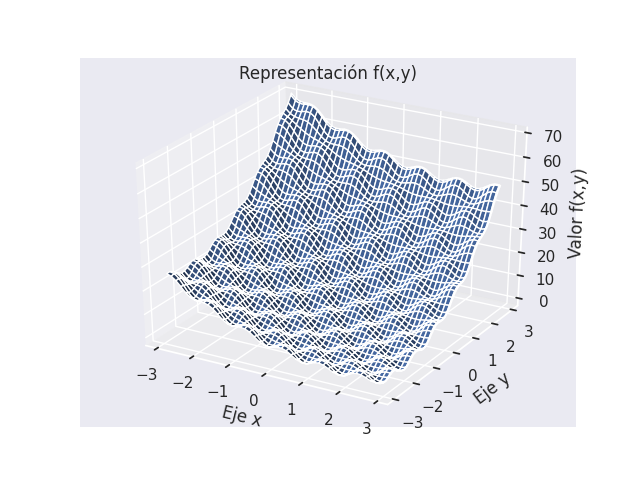
\includegraphics[width=0.75\textwidth]{f1}
    \caption{Función $f$}
    \label{fig:f1}
\end{figure}

\textbf{a) Usar gradiente descendente para minimizar esta función. Usar como punto inicial $(x_0 = 1, y_0 = -1)$, tasa de aprendizaje $\eta = 0,01$ y un máximo de 50 iteraciones.
Generar un gráfico de cómo desciende el valor de la función con las iteraciones. Repetir
el experimento pero usando $\eta = 0,1$, comentar las diferencias y su dependencia de $\eta$.}

Para usar el gradiente descendente necesitamos calcular el gradiente de la función que en este caso es:
\begin{align*}
\pdv{f}{x}(x,y) &= 2(x-2) + 4\pi \sin(2\pi y) \cos(2\pi x),\\
\pdv{f}{y}(x,y) &= 4(y+2)+4\pi \sin(2\pi x) \cos(2\pi y),\\
\grad{f}(x,y) &= \left(\pdv{f}{x}(x,y), \pdv{E}{y}(x,y)\right)^T\\
	      &= 2\left((x-2) + 2\pi \sin(2\pi y) \cos(2\pi x),\ 2(y+2)+2pi \sin(2\pi x) \cos(2\pi y)\right)^T.
\end{align*}

Tomaremos como parámetro, además de los impuestos para este experimento, \texttt{max\_iters} = 50.

\begin{figure}[H]
\centering
\begin{subfigure}{0.5\textwidth}
  \centering
  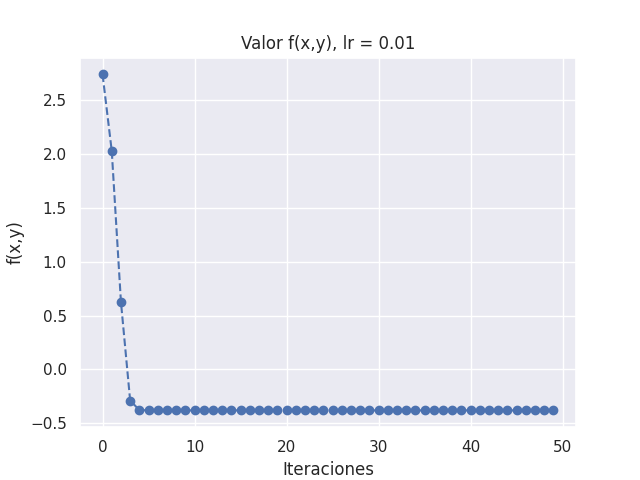
\includegraphics[width=1\linewidth]{1lr0_01}
  \caption{$\eta = 0.01$.}
  \label{fig:0.01}
\end{subfigure}%
\begin{subfigure}{.5\textwidth}
  \centering
  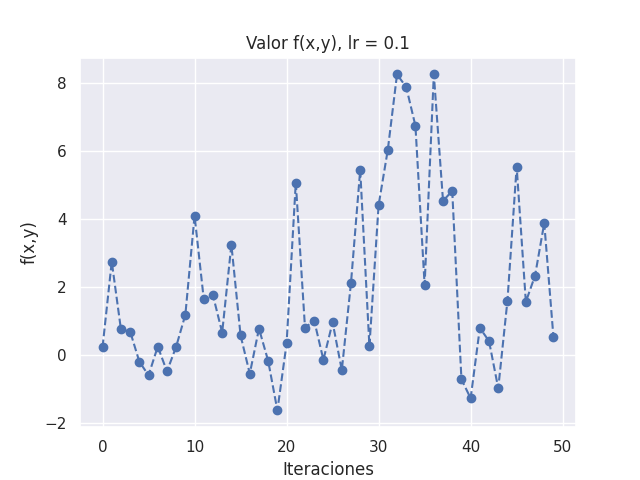
\includegraphics[width=1\linewidth]{1lr0_1}
  \caption{$\eta = 0.1$.}
  \label{fig:0.1}
\end{subfigure}
\caption{Valor de $f(x,y)$.}
\label{fig:test}
\end{figure}

En la Figura \ref{fig:0.01} vemos un gráfico de cómo desciende el valor de la función $f$ con las iteraciones cuando la tasa de aprendizaje es $0.01$, en la Figura \ref{fig:0.1} se ha generado el mismo gráfico para la tasa de aprendizaje $0.1$.

En un primer vistazo notamos que en la Figura \ref{fig:0.1} el valor de la función no es cada vez menor, su monotonía va cambiando. En el caso $\eta = 0.01$ la gráfica sí que es descendente, de hecho se estabiliza a partir de la quinta iteración. ¿A qué se debe esta diferencia?

La tasa de aprendizaje es un factor multiplicativo en la actualización del vector de pesos $w$, cuando vale 0.01 es pequeño y nos vamos desplazando en la dirección del gradiente poco a poco, hasta alcanzar un mínimo. Sin embargo, en el caso 0.1, ligeramente mayor, nos movemos dando pasos mayores en la dirección del gradiente, esto provoca que nos vayamos encontrando con diferentes mínimos y al aproximarnos a ellos, terminar alejándonos de uno para caer en otro. 

\textbf{b) Obtener el valor mínimo y los valores de las variables $(x, y)$ en donde se alcanzan cuando el punto de inicio se fija en: $(2,1, -2,1), (3, -3),(1,5, 1,5),(1, -1)$. Generar una
tabla con los valores obtenidos.}

Para esta experimentación se ha utilizado \texttt{lr} = 0.01 y \texttt{max\_iters} = 50.

\begin{table}[H]
\centering
\caption{Valor mínimo de $f$ y dónde se alcanza según el punto inicial.}
\label{tab:f}
\begin{tabular}{llll}
\toprule
$(x_0, y_0)$ & $x$ & $y$ & $f(x,y)$\\ \midrule
$(2.1, -2.1)$ & 2.2438049693647883 & -2.237925821486178 & -1.8200785415471563\\
$(3.0,-3.0)$ & 2.7309356482481055 & -2.7132791261667037 & -0.38124949743809955\\
$(1.5, 1.5)$ & 1.7779244744891156 & 1.032056872669696 & 18.042078009957635\\
$(1.0, -1.0)$ & 1.7566613758319838 & -0.8117887547719083 & 1.0333658794298513\\
\bottomrule
\end{tabular}
\end{table}

Observamos en la Tabla \ref{tab:f} que los valores mínimos alcanzados difieren según el punto inicial tomado. Si observamos la Figura \ref{fig:f1} notamos que el punto $(2.1, -2.1)$ tiene un valor de la función $f$ menor que los correspondientes al resto de valores iniciales, es por esto que al aplicar el algoritmo alcanza el mínimo global. Al ser el resto de puntos mayores, alcanzan mínimos  locales y se quedan estancados en ellos. El caso más destacable es el del punto $(1.5, 1.5)$, el valor mínimo obtenido al partir de este punto difiere enormemente de los obtenidos con el resto de puntos, esto se debe, como ya se ha comentado, a que se parte de un valor más alto de la función $f$ que queda atrapado en un mínimo local.

\subsection{¿Cuál sería su conclusión sobre la verdadera dificultad de encontrar el mínimo
global de una función arbitraria?}

Para encontrar un mínimo global de una función arbitraria creo que la dificultad no estriba en el algoritmo en sí, cuya posible dificultad es el cálculo de las derivadas parciales de las funciones, sino la determinación de los parámetros a utilizar.

En los ejercicios anteriores hemos probado epíricamente cómo, lo que a priori parecían ligeras variaciones en los parámetros, provocaron grandes diferencias en los resultados. Por un lado,  una tasa de aprendizaje mayor que la apropiada podría implicar que en cada iteración los valores de $w$ fueran oscilando sobre la función sin llegar a un óptimo. Mientras que, si este fuera demasiado pequeño, podríamos caer en un óptimo local. El punto inicial es también determinante en este sentido, si la función tiene varios mínimos locales y partimos cerca de uno que no sea el mínimo absoluto de la función, el algoritmo podría devolvernos como valor mínimo alguno de los mínimos locales.

Por tanto, la dificultad de este algoritmo consiste en encontrar la combinación de parámetros, desconocida, que nos permita alcanzar el mínimo global de la función, sin caer en óptimos locales ni quedarse oscilando.
\newpage
\section{Ejercicio sobre Regresión Lineal}
\textbf{Este ejercicio ajusta modelos de regresión a vectores de características extraidos de imágenes de digitos manuscritos. En particular se extraen dos característcas concretas: el valor medio del nivel de gris y simetría del número respecto de su eje vertical. Solo se seleccionarán para este ejercicio las imágenes de los números 1 y 5.}


\newpage
%%%%%%%%%%%%%%%%%%%%%%%%%%%%%%%%%%%%%%%%%%%%%%%%%%%%%%%%%%%%%%%%%%%
%       REFERENCIAS
%%%%%%%%%%%%%%%%%%%%%%%%%%%%%%%%%%%%%%%%%%%%%%%%%%%%%%%%%%%%%%%%%%%
\printbibliography
\end{document}
